% Graphic for TeX using PGF
% Title: /home/danielrb/Dropbox/Tesi/lin_adder/report/figures/vectorial_xor_bidecomposition.dia
% Creator: Dia v0.97.2
% CreationDate: Wed Nov 18 17:53:45 2015
% For: danielrb
% \usepackage{tikz}
% The following commands are not supported in PSTricks at present
% We define them conditionally, so when they are implemented,
% this pgf file will use them.
\ifx\du\undefined
  \newlength{\du}
\fi
\setlength{\du}{15\unitlength}
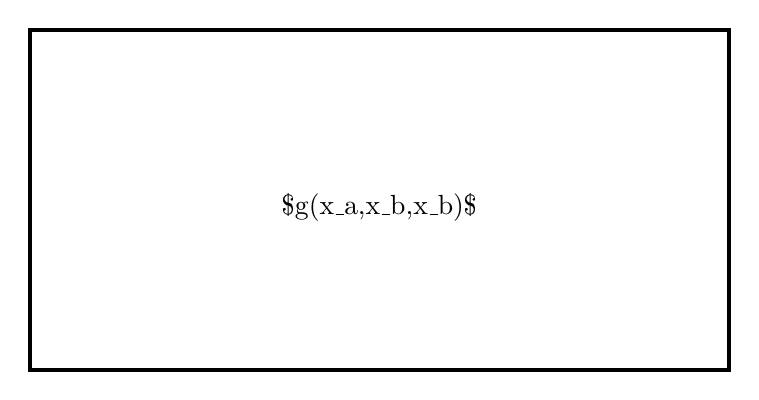
\begin{tikzpicture}
\pgftransformxscale{1.000000}
\pgftransformyscale{-1.000000}
\definecolor{dialinecolor}{rgb}{0.000000, 0.000000, 0.000000}
\pgfsetstrokecolor{dialinecolor}
\definecolor{dialinecolor}{rgb}{1.000000, 1.000000, 1.000000}
\pgfsetfillcolor{dialinecolor}
\definecolor{dialinecolor}{rgb}{1.000000, 1.000000, 1.000000}
\pgfsetfillcolor{dialinecolor}
\fill (20.100000\du,9.700000\du)--(20.100000\du,17.900000\du)--(36.950000\du,17.900000\du)--(36.950000\du,9.700000\du)--cycle;
\pgfsetlinewidth{0.100000\du}
\pgfsetdash{}{0pt}
\pgfsetdash{}{0pt}
\pgfsetmiterjoin
\definecolor{dialinecolor}{rgb}{0.000000, 0.000000, 0.000000}
\pgfsetstrokecolor{dialinecolor}
\draw (20.100000\du,9.700000\du)--(20.100000\du,17.900000\du)--(36.950000\du,17.900000\du)--(36.950000\du,9.700000\du)--cycle;
% setfont left to latex
\definecolor{dialinecolor}{rgb}{0.000000, 0.000000, 0.000000}
\pgfsetstrokecolor{dialinecolor}
\node at (28.525000\du,13.995000\du){\$g(x\_a,x\_b,x\_b)\$};
% setfont left to latex
\definecolor{dialinecolor}{rgb}{0.000000, 0.000000, 0.000000}
\pgfsetstrokecolor{dialinecolor}
\node[anchor=west] at (28.525000\du,13.800000\du){};
\end{tikzpicture}
